\documentclass[a4paper]{article}

\usepackage[english]{babel}
\usepackage{amsmath}
\usepackage{float}
\usepackage{amssymb}
\usepackage{dsfont}
\usepackage{graphicx}
\usepackage{listings}
\usepackage[hyphens]{url}
\usepackage{titling}
\usepackage{varwidth}
\usepackage{hyperref}
\usepackage{color} %red, green, blue, yellow, cyan, magenta, black, white
\definecolor{mygreen}{RGB}{28,172,0} % color values Red, Green, Blue
\definecolor{mylilas}{RGB}{170,55,241}



\usepackage{geometry}
 \geometry{
 a4paper,
 total={165mm,257mm},
 left=20mm,
 top=20mm,
 }

\title{Natural Computing\\Assignment 2}
\author{
  Christoph Schmidl\\ s4226887\\      \texttt{c.schmidl@student.ru.nl}
  \and
  Koen Vijverberg\\ s4132858\\     \texttt{koen.vijverberg@student.ru.nl}
  \and
  Alex\\	s4125304\\	\texttt{alex.kolmus@student.ru.nl}
}
\date{\today}

\begin{document}
\maketitle


\subsection*{Anomaly Detection using Negative Selection Algorithms}

\begin{enumerate}

	% Task 1	
	\item \textbf{Using the Negative Selection Algorithm}

	\begin{enumerate}
		\item[1.] Compute the area under the receiver operating characteristic cuve (AUC) to quantify how well the negative selection algorithm with parameters $n = 10, r = 4$ discriminates individual English string from Tagalog strings by using the files \textbf{english.train} for training and \textbf{english.test} as well as tagalog.test for testing.\\
		\textbf{Solution:}\\
		For $n = 10, r = 4$ the $AUC = 0.79$
		\begin{figure}[H]
	    \centering
  	    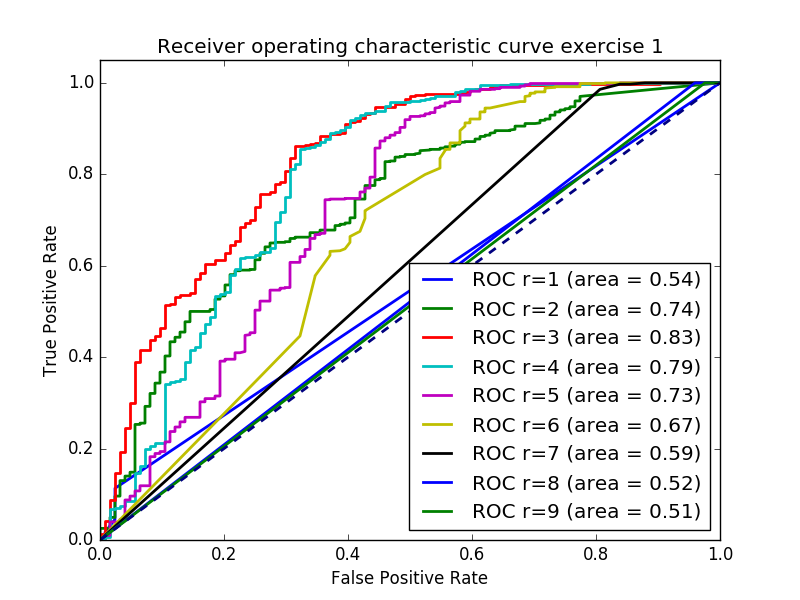
\includegraphics[width=0.8\textwidth]{images/ROC_exercise_1.png}
  	    \caption{The ROC curve plot for different values of $r$, the subsequent character matching parameter}
	    \end{figure}
		
		\item[2.] How does the AUC change when you modify the paramter $r$? Specifically, what behavior do you observe at $r = 1$ and $r = 9$ and how can you explain this behaviour? Which value of $r$ leads to the best discrimination?\\
		\textbf{Solution:}\\
		
		See figure 1, the AUC is in both edge cases ($r = 1$ and $r = 9$) close to 0.5, a.k.a. not better than random guessing. Best value is for $r = 3$ with an $AUC = 0.83$. \\
		
		\item[3.] The folder \textbf{lang} contains strings from 4 other languages. Determine which of these languages can be best discriminated from English using the negative selection algorithm, and for which of the languages this is most difficult. Can you explain your findings?\\
		\textbf{Solution:}\\
		
		Xhosa is easiest discriminated (best AUC score), worst is middle-english, which seems reasonable because it is probably similar to the normal english language.
		\begin{figure}[H]
	    \centering
  	    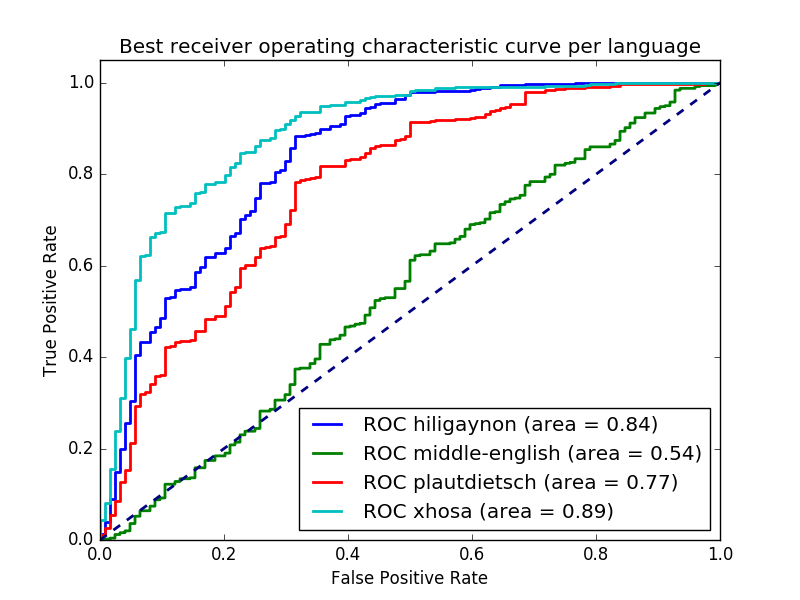
\includegraphics[width=0.8\textwidth]{images/ROC_exercise_1_langs.png}
  	    \caption{Best ROC curves per language}
	    \end{figure}
			
	\end{enumerate}		
	
	
	% Task 2	
	\item \textbf{Intrusion Detection for Unix Processes}
	
	Use negative selection to detect the anomalous sequences in the system calls datasets! Perform an AUC analysis to evaluate the quality of your classification.\\There are two importan differences to the "toy example".
	
	\begin{enumerate}
		\item[1.] The data format differs slightly, with the classification being stored in the separate \textbf{.labels} rather than having two different files for normal and anomalous data.	
		\item[2.] More importantly, the sequences stored in the files are no longer of a fixed length. For training, this means that you will need to pre-process each sequence to a set of fixed-length chunks (for instance, you could use all substrings of a fixed length, or all non-overlapping substrings of a fixed length). For classification, you also need to split the sequences into chunks, compute the number of matching patterns for each chunk separately, and merge these counts together to a composite anomaly score (for instance, you could average the individual counts).
	\end{enumerate}		

Choose the parameters $n$ and $r$ for the negative selection algorithm yourself. You can use the parameters from the language example as a starting point.\\
\textbf{Solution:}\\

\end{enumerate}




\end{document}